\newpage
\section{Graph Theory}
\label{sec:graphs}

\subsection{Basic definitions}
\label{sec:11-1}
% CN 11.1

\begin{definition}[Graph]
A \emph{graph} $G=(V,E)$ consists of a set $V$ of \emph{vertices} and a set $E$ of \emph{edges}, each edge being an unordered pair $\{v,w\}$ of vertices.
\end{definition}

\begin{definition}[Adjacent, neighbour, incident]
$v$ and $w$ are \emph{adjacent}, written $v\sim w$, if $\{v,w\}\in E$; otherwise $v\not\sim w$. Then each is a \emph{neighbour} of the other, and both are \emph{incident} with the edge $\{v,w\}$ (they are its \emph{endpoints}). The \emph{neighbourhood} $N(v)$ is the set of all neighbours of $v$.
\end{definition}

\begin{definition}[Isolated vertex, leaf]
$v$ is \emph{isolated} if $N(v)=\emptyset$, and a \emph{leaf} if $|N(v)|=1$.
\end{definition}

\begin{example}
Let $V=\{a,b,c,d,e,f,g\}$ and $E=\{\{a,b\},\{a,c\},\{b,c\},\{c,d\},\{f,g\}\}$: seven vertices and five edges. Here $a\sim b$, $a\sim c$, $b\sim c$, $c\sim d$, $f\sim g$, and every other pair is non-adjacent, e.g.\ $d\not\sim f$. Also $N(c)=\{a,b,d\}$.
\end{example}

\begin{center}
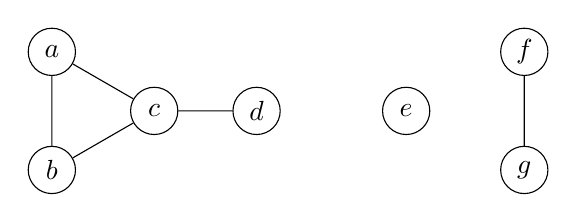
\begin{tikzpicture}[every node/.style={circle,draw,fill=white,inner sep=1.5pt,minimum size=6mm}]
\node (a) at (0,1.5) {$a$};
\node (b) at (0,0) {$b$};
\node (c) at (1.3,0.75) {$c$};
\node (d) at (2.6,0.75) {$d$};
\node (e) at (4.5,0.75) {$e$};
\node (f) at (6,1.5) {$f$};
\node (g) at (6,0) {$g$};
\draw (a)--(b) (a)--(c) (b)--(c) (c)--(d) (f)--(g);
\end{tikzpicture}
\end{center}
\begin{center}
\small $e$ is isolated; $d,f,g$ are leaves; $\{a,b,c,d\}$, $\{e\}$, $\{f,g\}$ are the three components (\S\ref{sec:11-9})
\end{center}

\begin{note}[A graph is not its drawing]
The graph is just the pair $(V,E)$. Positions of dots, lengths of lines and crossings in a picture carry no information; many different drawings show the same graph.
\end{note}

\subsection{Types of graphs}
\label{sec:11-2}
% CN 11.2

\begin{definition}[Simple graph]
$G$ is \emph{simple} if it has no loops (edges $\{v,v\}$) and no multiple edges.
\end{definition}

\begin{note}[Relaxations]
A \emph{multigraph} allows multiple edges; a \emph{pseudograph} also allows loops. In a \emph{directed graph} the edges are ordered pairs $(v,w)$ (\emph{arcs}), e.g.\ for one-way streets. In a \emph{weighted graph} each edge carries a number, such as a distance or cost.
\end{note}

\begin{center}
\begin{tikzpicture}[every node/.style={circle,draw,fill=white,inner sep=1.5pt,minimum size=6mm}, >={Stealth[length=2mm]}]
\node (v1) at (0,0) {$v_1$};
\node (v2) at (2,0.8) {$v_2$};
\node (v3) at (2,-0.8) {$v_3$};
\node (v4) at (4,0) {$v_4$};
\draw[->] (v1)--(v2);
\draw[->] (v1)--(v3);
\draw[->] (v2)--(v4);
\draw[->] (v3)--(v4);
\draw[->] (v2) to[bend left] (v3);
\draw[->] (v4) to[out=150,in=210,looseness=8] (v4);
\end{tikzpicture}
\qquad
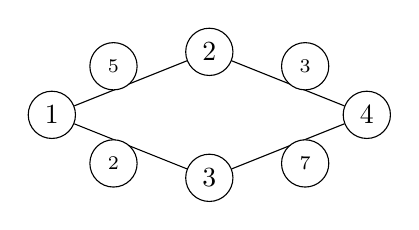
\begin{tikzpicture}[every node/.style={circle,draw,fill=white,inner sep=1.5pt,minimum size=6mm}]
\node (w1) at (0,0) {$1$};
\node (w2) at (2,0.8) {$2$};
\node (w3) at (2,-0.8) {$3$};
\node (w4) at (4,0) {$4$};
\draw (w1)--(w2) node[midway,above left,font=\scriptsize] {$5$};
\draw (w1)--(w3) node[midway,below left,font=\scriptsize] {$2$};
\draw (w2)--(w4) node[midway,above right,font=\scriptsize] {$3$};
\draw (w3)--(w4) node[midway,below right,font=\scriptsize] {$7$};
\end{tikzpicture}
\end{center}
\begin{center}
\small Directed graph (left, with a self-loop at $v_4$) and weighted graph (right)
\end{center}

\begin{definition}[Complement]
For a simple graph $G=(V,E)$, the \emph{complement} is $\overline G=(V,\overline E)$, where $\overline E=\{\{v,w\}: v\neq w,\ \{v,w\}\notin E\}$.
\end{definition}

\begin{proposition}
For a simple graph $G$ on $n$ vertices, \ $|E(\overline G)| = \binom n2 - |E(G)|$.
\end{proposition}
\begin{proof}
Each of the $\binom n2$ pairs of distinct vertices is an edge of exactly one of $G$ and $\overline G$.
\end{proof}

\begin{definition}[Wheel graph]
$W_n$ is the cycle $C_n$ (the \emph{rim}) together with one extra vertex (the \emph{hub}) adjacent to all $n$ rim vertices.
\end{definition}

\subsection{Subgraphs}
\label{sec:11-5}
% CN 11.5

\begin{definition}[Subgraph]\label{def:subgraph}
$H=(V_H,E_H)$ is a \emph{subgraph} of $G=(V,E)$, written $H\le G$, if $V_H\subseteq V$ and $E_H\subseteq E$ (every edge of $H$ having both endpoints in $V_H$). It is a \emph{proper} subgraph, $H<G$, if also $H\ne G$.
\end{definition}

\begin{example}
For the graph $G$ of \S\ref{sec:11-1}, let $F=(U,D)$ with $U=\{a,b,c,e,g\}$ and $D=\{\{a,b\},\{a,c\}\}$. Then $F\le G$, and in fact $F<G$. Note that $\{b,c\}$ is left out even though $b,c\in U$.
\end{example}

\begin{definition}[Induced subgraph]\label{def:induced-subgraph}
The subgraph \emph{induced} by $S\subseteq V$, written $G[S]$, has vertex set $S$ and \emph{all} edges of $G$ with both endpoints in $S$.
\end{definition}

\begin{center}
\begin{tikzpicture}[every node/.style={circle,draw,fill=white,inner sep=1.5pt,minimum size=6mm}]
\node (p) at (0,1) {$p$};
\node (q) at (1.3,1.6) {$q$};
\node (r) at (1.3,0.4) {$r$};
\node (s) at (2.6,1) {$s$};
\draw[thick] (p)--(q) (p)--(r) (q)--(r) (q)--(s) (r)--(s);
\begin{scope}[on background layer]
\filldraw[fill=blue!10,draw=blue,rounded corners] (-0.5,0.2) rectangle (2,2.1);
\end{scope}
\end{tikzpicture}
\end{center}
\begin{center}
\small The subgraph induced by $\{p,q,r\}$ (shaded): it includes \emph{every} edge among them, $\{p,q\},\{p,r\},\{q,r\}$
\end{center}

\begin{note}[Induced vs.\ ordinary subgraph]
Every induced subgraph is a subgraph, but not conversely. For a subgraph $H$ we only know $E_H\subseteq E(G[V_H])$, while $H$ is induced exactly when equality holds, $H=G[V_H]$. The graph $F$ above is not induced, since it omits $\{b,c\}$.
\end{note}

\subsection{Some special graphs}
\label{sec:11-6}
% CN 11.6

\begin{definition}[Standard families]
\label{def:families}
\begin{itemize}
    \item $K_n$ (\emph{complete graph}): $n$ vertices, every pair adjacent.
    \item $\overline{K_n}$ (\emph{null graph}): $n$ vertices, no edges.
    \item $C_n$ (\emph{cycle}): $v_1\sim v_2\sim\cdots\sim v_n\sim v_1$, for $n\ge3$.
    \item $P_{n-1}$ (\emph{path of length $n-1$}): vertices $v_1,\dots,v_n$ with $v_i\sim v_j$ iff $|i-j|=1$.
    \item $K_{m,n}$ (\emph{complete bipartite}): $V=A\sqcup B$ with $|A|=m$, $|B|=n$, and $v\sim w$ iff one is in $A$ and the other in $B$.
    \item $Q_n$ (\emph{hypercube}): $V=\{0,1\}^n$, with $v\sim w$ iff they differ in exactly one coordinate.
\end{itemize}
\end{definition}

\begin{proposition}
\label{thm:edge-counts}
$|E(K_n)| = \binom n2$, \ $|E(\overline{K_n})| = 0$, \ $|E(P_{n-1})| = n-1$, \ $|E(Q_n)| = n\cdot2^{n-1}$.
\end{proposition}
\begin{proof}
In $K_n$ the edges are exactly the unordered pairs of distinct vertices, so there are $\binom n2$. The null graph has no edges. The edges of $P_{n-1}$ are $\{v_i,v_{i+1}\}$ for $i=1,\dots,n-1$. In $Q_n$ every vertex has degree $n$ (flip any one of the $n$ coordinates), so by the handshaking lemma (Theorem~\ref{thm:handshake}) $|E|=n\cdot2^n/2=n2^{n-1}$.
\end{proof}

\begin{center}
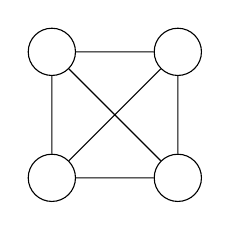
\begin{tikzpicture}[every node/.style={circle,draw,fill=white,inner sep=1.5pt,minimum size=6mm}]
\node (p0) at (0,0) {};
\node (p1) at (1.6,0) {};
\node (p2) at (1.6,1.6) {};
\node (p3) at (0,1.6) {};
\draw (p0)--(p1) (p1)--(p2) (p2)--(p3) (p3)--(p0) (p0)--(p2) (p1)--(p3);
\end{tikzpicture}
\qquad
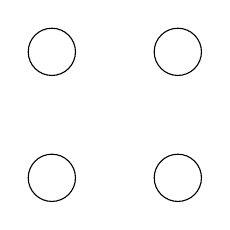
\begin{tikzpicture}[every node/.style={circle,draw,fill=white,inner sep=1.5pt,minimum size=6mm}]
\node at (0,0) {};
\node at (1.6,0) {};
\node at (1.6,1.6) {};
\node at (0,1.6) {};
\end{tikzpicture}
\qquad
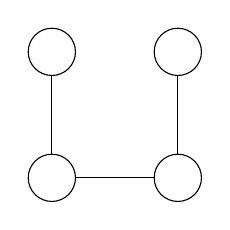
\begin{tikzpicture}[every node/.style={circle,draw,fill=white,inner sep=1.5pt,minimum size=6mm}]
\node (p0) at (0,0) {};
\node (p1) at (1.6,0) {};
\node (p2) at (1.6,1.6) {};
\node (p3) at (0,1.6) {};
\draw (p3)--(p0) (p0)--(p1) (p1)--(p2);
\end{tikzpicture}
\qquad
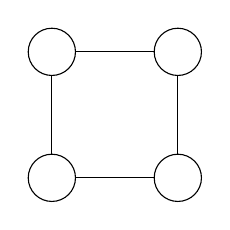
\begin{tikzpicture}[every node/.style={circle,draw,fill=white,inner sep=1.5pt,minimum size=6mm}]
\node (p0) at (0,0) {};
\node (p1) at (1.6,0) {};
\node (p2) at (1.6,1.6) {};
\node (p3) at (0,1.6) {};
\draw (p0)--(p1) (p1)--(p2) (p2)--(p3) (p3)--(p0);
\end{tikzpicture}
\end{center}
\begin{center}
\small $K_4$, \ $\overline{K_4}$, \ $P_3$, \ $C_4$ (left to right)
\end{center}

\begin{center}
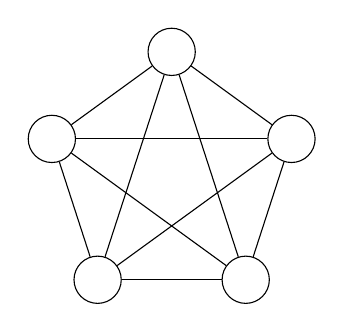
\begin{tikzpicture}[every node/.style={circle,draw,fill=white,inner sep=1.5pt,minimum size=6mm}]
\foreach \i in {0,...,4} {
  \node (v\i) at ({90+\i*72}:1.6) {};
}
\foreach \i in {0,...,4} {
  \foreach \j in {0,...,4} {
    \ifnum\i<\j
      \draw (v\i)--(v\j);
    \fi
  }
}
\end{tikzpicture}
\qquad
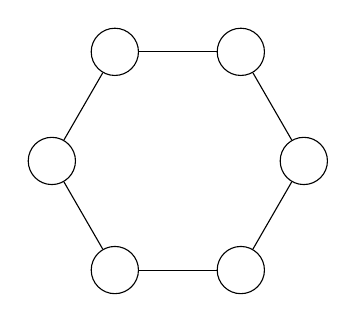
\begin{tikzpicture}[every node/.style={circle,draw,fill=white,inner sep=1.5pt,minimum size=6mm}]
\foreach \i in {0,...,5} {
  \node (c\i) at ({60*\i}:1.6) {};
}
\foreach \i in {0,...,5} {
  \pgfmathtruncatemacro{\j}{mod(\i+1,6)}
  \draw (c\i)--(c\j);
}
\end{tikzpicture}
\end{center}
\begin{center}
\small $K_5$ (left) and $C_6$ (right)
\end{center}

\begin{center}
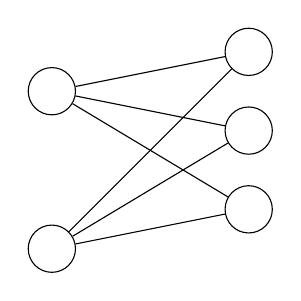
\begin{tikzpicture}[every node/.style={circle,draw,fill=white,inner sep=1.5pt,minimum size=6mm}]
\node (a1) at (0,1) {};
\node (a2) at (0,-1) {};
\node (b1) at (2.5,1.5) {};
\node (b2) at (2.5,0.5) {};
\node (b3) at (2.5,-0.5) {};
\foreach \a in {a1,a2} {
  \foreach \b in {b1,b2,b3} {
    \draw (\a)--(\b);
  }
}
\end{tikzpicture}
\qquad
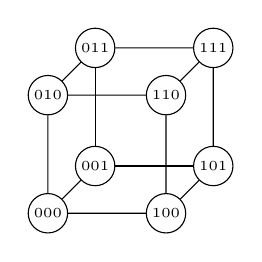
\begin{tikzpicture}[every node/.style={circle,draw,fill=white,inner sep=1pt,minimum size=5mm,font=\tiny}]
\node (000) at (0,0) {000};
\node (100) at (1.5,0) {100};
\node (010) at (0,1.5) {010};
\node (001) at (0.6,0.6) {001};
\node (110) at (1.5,1.5) {110};
\node (101) at (2.1,0.6) {101};
\node (011) at (0.6,2.1) {011};
\node (111) at (2.1,2.1) {111};
\draw (000)--(100) (000)--(010) (000)--(001);
\draw (100)--(110) (100)--(101);
\draw (010)--(110) (010)--(011);
\draw (001)--(101) (001)--(011);
\draw (110)--(111) (101)--(111) (011)--(111);
\end{tikzpicture}
\end{center}
\begin{center}
\small $K_{2,3}$ (left) and $Q_3$ (right)
\end{center}

\subsection{Degree}
\label{sec:11-7}
% CN 11.7

\begin{definition}[Degree]
\label{def:degree}
The \emph{degree} of $v$ is $\deg(v) = |N(v)|$, the number of neighbours of $v$. Write $\deg_G(v)$ when the graph needs to be specified.
\end{definition}

\begin{note}[Isolated vertices and leaves]
In a simple graph, $\deg(v)$ is also the number of edges at $v$. So $v$ is isolated iff $\deg(v)=0$, and a leaf iff $\deg(v)=1$. In the graph of \S\ref{sec:11-1}, $\deg(c)=3$, $\deg(a)=\deg(b)=2$, $\deg(d)=\deg(f)=\deg(g)=1$, $\deg(e)=0$.
\end{note}

\begin{theorem}[Handshaking lemma]
\label{thm:handshake}
For every graph, \ $\displaystyle\sum_{v\in V} \deg(v) = 2|E|$.
\end{theorem}
\begin{proof}
Each edge $\{v,w\}$ contributes exactly $1$ to $\deg(v)$ and $1$ to $\deg(w)$, so $2$ to the sum. Adding over all edges gives $2|E|$.
\end{proof}
\begin{proof}[Alternative proof, via the adjacency matrix]
The number of $1$'s in the column of $v$ is $\deg(v)$, so $\sum_v\deg(v)$ is the total number of $1$'s in $A$. Each edge $\{v,w\}$ gives exactly two of them, $A_{vw}$ and $A_{wv}$, so the total is $2|E|$.
\end{proof}

\begin{example}
In the graph of \S\ref{sec:11-1}, the degrees add up to $2+2+3+1+0+1+1=10=2\cdot5$.
\end{example}

\begin{corollary}
\label{cor:odd-degree}
In every graph, the number of vertices of odd degree is even.
\end{corollary}
\begin{proof}
The sum $\sum_v\deg(v)=2|E|$ is even. Split it into the sum over even-degree vertices, which is even, and the sum over odd-degree vertices, which must therefore also be even. A sum of $k$ odd numbers has the same parity as $k$, so $k$ is even.
\end{proof}

\begin{corollary}[Average degree]
\label{cor:avg-degree}
A graph with $n$ vertices and $m$ edges has average degree $\dfrac1n\sum_{v}\deg(v) = \dfrac{2m}{n}$.
\end{corollary}
\begin{proof}
Divide Theorem~\ref{thm:handshake} by $n$.
\end{proof}

\begin{note}[Range of the average]
Since $0\le\deg(v)\le n-1$, the average degree lies between $0$ (the null graph $\overline{K_n}$) and $n-1$ (the complete graph $K_n$). The formula $2m/n$ uses only the global counts $n$ and $m$, yet tells us about local structure.
\end{note}

\begin{note}[Directed graphs (extra)]
For a directed graph, let $\deg^-(v)$ and $\deg^+(v)$ be the in-degree and out-degree of $v$. Each arc $(v,w)$ contributes $1$ to $\deg^+(v)$ and $1$ to $\deg^-(w)$, so $\sum_v\deg^-(v)=\sum_v\deg^+(v)=|E|$.
\end{note}

\bigskip
\begin{theorem}[CN Thm 56]
\label{thm:equal-degree}
In every graph with at least two vertices, there are two vertices with the same degree.
\end{theorem}
\begin{proof}
Let $G$ have $n\ge2$ vertices. The possible degrees are $0,1,\dots,n-1$, which is $n$ values. We use proof by cases, depending on whether $G$ has a vertex of degree $n-1$.

\textbf{Case 1} ($G$ has no vertex of degree $n-1$): Then the degrees lie in $\{0,\dots,n-2\}$, which has only $n-1$ values. With $n$ vertices, two of them must share a degree.

\textbf{Case 2} ($G$ has a vertex $v$ of degree $n-1$): Then $v$ is adjacent to every other vertex, so no vertex has degree $0$. The degrees lie in $\{1,\dots,n-1\}$, again only $n-1$ values for $n$ vertices, so two vertices share a degree.
\end{proof}

\begin{note}[The key observation]
Degrees $0$ and $n-1$ cannot both occur: a vertex of degree $n-1$ is adjacent to everything, and a vertex of degree $0$ to nothing. So the $n$ vertices have at most $n-1$ values available.
\end{note}

\begin{note}[Necessary conditions on degree lists]
For $d_1,\dots,d_n$ (with $0\le d_i\le n-1$) to be the degrees of a graph on $n$ vertices, it is necessary that $\sum_i d_i$ is even (Theorem~\ref{thm:handshake}), that the number of odd $d_i$ is even (Corollary~\ref{cor:odd-degree}), and, if $n\ge2$, that the $d_i$ are not all different (Theorem~\ref{thm:equal-degree}). These conditions are not sufficient, as the next example shows.
\end{note}

\begin{example}
The list $3,3,1,1$ passes all three tests, but no graph on $4$ vertices has these degrees: the two vertices of degree $3$ would each be adjacent to all other vertices, so the remaining two vertices would have degree at least $2$, not $1$.
\end{example}

\subsection{Representing graphs}
\label{sec:11-4}
% CN 11.4

\subsubsection{Edge list}
\begin{definition}[Edge list]
The \emph{edge list} of $G$ lists the vertex set and every edge $\{v,w\}$ explicitly.
\end{definition}

\subsubsection{Adjacency matrix}
\begin{definition}[Adjacency matrix]
For $V=\{v_1,\dots,v_n\}$, the \emph{adjacency matrix} is the $n\times n$ matrix $A$ with $A_{ij}=1$ if $v_i\sim v_j$, and $A_{ij}=0$ otherwise.
\end{definition}

\begin{example}
For the graph of \S\ref{sec:11-1}, restricted to $\{a,b,c,d,e\}$ in that order,
\[
A =
\begin{pmatrix}
0 & 1 & 1 & 0 & 0 \\
1 & 0 & 1 & 0 & 0 \\
1 & 1 & 0 & 1 & 0 \\
0 & 0 & 1 & 0 & 0 \\
0 & 0 & 0 & 0 & 0
\end{pmatrix}.
\]
For instance $a\sim c$ because the entry in row $a$, column $c$ is $1$; the last row is all zero because $e$ is isolated.
\end{example}

\begin{note}[Shape of the matrix]
$A$ is symmetric because edges are unordered, and its diagonal is all $0$ because a simple graph has no loops. It is exactly the zero-one matrix of the adjacency relation (\S\ref{sec:2-6}).
\end{note}

\subsubsection{Adjacency list}
\begin{definition}[Adjacency list]
\label{def:adjacency-list}
For each vertex $v$, store the list $N(v)$ of its neighbours. The \emph{adjacency list} of $G$ is the collection of these $n$ lists.
\end{definition}

\begin{example}
The graph of \S\ref{sec:11-1} has adjacency list
\[
a: b,c \qquad b: a,c \qquad c: a,b,d \qquad d: c \qquad e: \text{--} \qquad f: g \qquad g: f
\]
From it we read off at once that $N(c)=\{a,b,d\}$, that $e$ has no neighbours, and that the leaves are $d,f,g$.
\end{example}

\begin{note}[Most common in practice]
The adjacency list is the most widely used representation in computers: it is compact, and it makes searching the neighbourhood of a vertex fast, which many graph algorithms need.
\end{note}

\subsubsection{Incidence matrix}
\begin{definition}[Incidence matrix]
\label{def:incidence-matrix}
For $V=\{v_1,\dots,v_n\}$ and $E=\{e_1,\dots,e_m\}$, the \emph{incidence matrix} $M$ is the $n\times m$ matrix with $M_{ij}=1$ if $v_i$ is incident with $e_j$, and $M_{ij}=0$ otherwise.
\end{definition}

\begin{note}[Columns]
Each column of $M$ contains exactly two $1$'s, one for each endpoint of that edge.
\end{note}

\begin{proposition}[Incidence matrix and adjacency matrix (extra)]
\label{prop:MMT}
Let $G$ be a simple graph with adjacency matrix $A$ and incidence matrix $M$, and let $D=\operatorname{diag}\bigl(\deg(v_1),\dots,\deg(v_n)\bigr)$. Then $MM^{\mathsf T}=A+D$.
\end{proposition}
\begin{proof}
By the definition of matrix multiplication, $(MM^{\mathsf T})_{ij}=\sum_{k}M_{ik}M_{jk}$ counts the edges incident with both $v_i$ and $v_j$. If $i=j$, this counts the edges at $v_i$, which is $\deg(v_i)=D_{ii}$. If $i\ne j$, the only possible such edge is $\{v_i,v_j\}$, so the count is $1$ if $v_i\sim v_j$ and $0$ otherwise, which is $A_{ij}$.
\end{proof}

\begin{note}[Comparison of representations]
Up to a constant factor:
\[
\begin{array}{l|cccc}
 & \text{edge list} & \text{adjacency list} & \text{adjacency matrix} & \text{incidence matrix}\\\hline
\text{space} & |E| & n+|E| & n^2 & n|E|\\
\text{test } v\sim w & \text{scan list} & \deg(v) & 1 & \text{scan row}\\
\text{list } N(v) & \text{scan list} & \deg(v) & n & \text{scan row}
\end{array}
\]
Sparse graphs favour lists; dense graphs, or computations using matrix algebra, favour matrices.
\end{note}

\subsection{Graphs and relations}
\label{sec:11-3}
% CN 11.3

\begin{proposition}
Simple graphs on $V$ correspond exactly to irreflexive symmetric binary relations on $V$.
\end{proposition}
\begin{proof}
Given a simple graph $G=(V,E)$, define $R\subseteq V\times V$ by $(v,w)\in R$ iff $\{v,w\}\in E$. Then $R$ is irreflexive, since there are no loops, and symmetric, since $\{v,w\}=\{w,v\}$. Conversely, an irreflexive symmetric $R$ on $V$ gives the simple graph with $E=\{\{v,w\}:(v,w)\in R\}$, and these two constructions undo each other.
\end{proof}

\begin{note}[Dropping the conditions]
Dropping irreflexivity allows loops; dropping symmetry gives directed graphs. An arbitrary binary relation on $V$ (\S\ref{sec:2-13}) is the same thing as a directed graph with loops allowed.
\end{note}

\subsection{Walks, paths and cycles}
\label{sec:11-8}
% CN 11.8

\begin{definition}[Walk, closed walk]
\label{def:walk-closed}\label{def:walk}
A \emph{walk} from $v$ to $w$ is a sequence $v_0,e_1,v_1,e_2,\dots,e_k,v_k$ of vertices and edges with $v_0=v$, $v_k=w$, and $e_i=\{v_{i-1},v_i\}$ for each $i$. Its \emph{length} is $k$, the number of edges. The walk is \emph{closed} if $v_0=v_k$.
\end{definition}

\begin{note}[Two freedoms]
A walk may visit a vertex more than once, and may use an edge more than once, in either direction. The shortest walk has length $0$: a single vertex and no edges. In a simple graph a walk is determined by its vertices alone, so we usually write just $v_0,v_1,\dots,v_k$.
\end{note}

\begin{center}
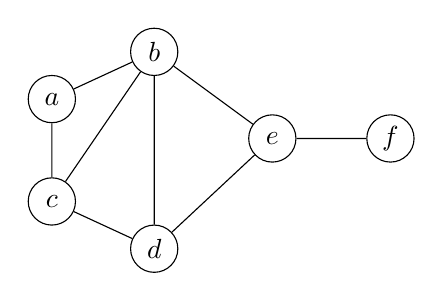
\begin{tikzpicture}[every node/.style={circle,draw,fill=white,inner sep=1.5pt,minimum size=6mm}]
\node (a) at (0,1) {$a$};
\node (b) at (1.3,1.6) {$b$};
\node (c) at (0,-0.3) {$c$};
\node (d) at (1.3,-0.9) {$d$};
\node (e) at (2.8,0.5) {$e$};
\node (f) at (4.3,0.5) {$f$};
\draw (a)--(b) (a)--(c) (b)--(c) (b)--(d) (c)--(d) (b)--(e) (d)--(e) (e)--(f);
\end{tikzpicture}
\end{center}

\begin{example}
In the graph above:
\begin{itemize}
    \item $a,b,d,e,f$ is a walk of length $4$ from $a$ to $f$;
    \item $a,b,d,c,b,e$ is a walk of length $5$ (it revisits $b$);
    \item $b,e,f,e,d$ is a walk of length $4$ (it uses $\{e,f\}$ twice);
    \item $a,b,c,a$ is a closed walk of length $3$, and $a,b,c,b,c,a$ is one of length $5$;
    \item $c$ alone is a walk of length $0$.
\end{itemize}
\end{example}

\begin{definition}[Trail, path, cycle]
\label{def:trail-path-cycle}
A walk is a \emph{trail} if no edge is used more than once; a \emph{closed trail} is a trail with $v_0=v_k$. A \emph{path} is a trail with no repeated vertex. A \emph{cycle} is a closed trail with no repeated vertex other than $v_0=v_k$.
\end{definition}

\begin{example}
In the graph above, $a,b,c,a$ and $a,c,b,d,e,b,a$ are closed trails (the second revisits $b$, so it is not a cycle). $a,b,d,e,f$ is a path, but not a shortest one: the shortest path from $a$ to $f$ is $a,b,e,f$, of length $3$. Shortest paths need not be unique: $a,b,d$ and $a,c,d$ are both shortest paths from $a$ to $d$.
\end{example}

\begin{note}[Each notion restricts the last]
Walk $\supseteq$ trail $\supseteq$ path: a trail gives up reusing edges, and a path also gives up reusing vertices. A cycle is \emph{not} a ``closed path'', since a path of length $\ge1$ cannot be closed. In a simple graph a cycle has length at least $3$: there are no loops, and $u,v,u$ uses the edge $\{u,v\}$ twice.
\end{note}

\begin{lemma}[Shortest walk is a path]
\label{lem:shortest-path}
If there is a walk from $v$ to $w$, then every shortest walk from $v$ to $w$ is a path. Hence $v$ and $w$ are joined by a walk iff they are joined by a path.
\end{lemma}
\begin{proof}
Let $v_0,\dots,v_k$ be a shortest walk from $v$ to $w$, and suppose, for contradiction, that $v_i=v_j$ for some $i<j$. Cutting out the part between them gives $v_0,\dots,v_i,v_{j+1},\dots,v_k$, which is still a walk from $v$ to $w$ (as $v_i=v_j\sim v_{j+1}$) but is shorter, by $j-i$. This contradicts minimality. So no vertex repeats, hence no edge repeats, and the walk is a path.
\end{proof}

\begin{definition}[Distance]
\label{def:distance}
If $v$ and $w$ are joined by a walk, the \emph{distance} $d(v,w)$ is the length of a shortest path between them (equivalently, of a shortest walk, by Lemma~\ref{lem:shortest-path}). Otherwise $d(v,w)=\infty$.
\end{definition}

\bigskip
\begin{theorem}[CN Thm 60]
\label{thm:odd-closed-walk}
A graph has a closed walk of odd length if and only if it has a cycle of odd length.
\end{theorem}
\begin{proof}
($\Leftarrow$) Every cycle is a closed walk of the same length.

($\Rightarrow$) Let $W=v_0,\dots,v_k$ be a \emph{shortest} closed walk of odd length $k$. Since there are no loops, $k\ge3$. We claim that no vertex repeats in $W$ apart from $v_0=v_k$.

Suppose, for contradiction, that $v_i=v_j$ with $0\le i<j\le k-1$. Splitting $W$ at this vertex gives two closed walks, $v_i,\dots,v_j$ of length $j-i$, and $v_j,\dots,v_{k-1},v_0,\dots,v_i$ of length $k-(j-i)$. Both lengths are between $1$ and $k-1$, and they add up to the odd number $k$, so one of them is odd. That is an odd closed walk shorter than $W$, a contradiction.

So $W$ repeats no vertex except $v_0=v_k$. Then it repeats no edge either (as $k\ge3$), so $W$ is a cycle of odd length.
\end{proof}

\begin{note}[The ``even'' version fails]
$K_2$ has the closed walk $v,w,v$ of even length $2$ but no cycle at all. The proof breaks because an even length can split as odd $+$ odd, so no shorter \emph{even} closed walk need appear.
\end{note}

\subsubsection*{Counting walks with the adjacency matrix}

\begin{theorem}[Counting walks via matrix powers (extra)]
\label{thm:walks}
Let $A$ be the adjacency matrix of $G$. For every $r\ge1$, $(A^r)_{ij}$ is the number of walks of length $r$ from $v_i$ to $v_j$.
\end{theorem}
\begin{proof}
We use induction on $r$.

\textbf{Base case} ($r=1$): A walk of length $1$ from $v_i$ to $v_j$ is a single edge, so there is one if $v_i\sim v_j$ and none otherwise. That count is $A_{ij}$.

\textbf{Inductive step}: Assume $(A^r)_{ik}$ counts the walks of length $r$ from $v_i$ to $v_k$, for all $i,k$. Classify the walks of length $r+1$ from $v_i$ to $v_j$ by their second-to-last vertex $v_k$. Such a walk is a walk of length $r$ from $v_i$ to $v_k$, which can be chosen in $(A^r)_{ik}$ ways by the inductive hypothesis, followed by a final step $v_k\to v_j$, which exists ($1$ way) iff $A_{kj}=1$. So there are $(A^r)_{ik}A_{kj}$ walks with second-to-last vertex $v_k$. Every walk has exactly one second-to-last vertex, so adding over $k$ gives $\sum_{k}(A^r)_{ik}A_{kj}$, which is the $(i,j)$ entry of $A^rA=A^{r+1}$.

By the Principle of Mathematical Induction, the claim holds for all $r\ge1$.
\end{proof}

\begin{note}[Walks, not paths]
The theorem counts walks, which may repeat vertices. It also holds for $r=0$: $A^0=I$, and the only walk of length $0$ from $v_i$ ends at $v_i$.
\end{note}

\begin{example}
For the triangle on $\{a,b,c\}$,
\[
A=\begin{pmatrix}0&1&1\\1&0&1\\1&1&0\end{pmatrix},\qquad
A^2=\begin{pmatrix}2&1&1\\1&2&1\\1&1&2\end{pmatrix}.
\]
$(A^2)_{aa}=2$ counts the walks $a,b,a$ and $a,c,a$, and $(A^2)_{ab}=1$ counts the walk $a,c,b$.
\end{example}

\subsection{Connectivity}
\label{sec:11-9}
% CN 11.9

\begin{definition}[Connected graph, component]
Vertices $v,w$ are \emph{connected} if there is a path (equivalently, a walk) between them. $G$ is \emph{connected} if every pair of vertices is connected. A \emph{component} of $G$ is a maximal connected subgraph.
\end{definition}

\begin{proposition}
Being connected is an equivalence relation on $V$, and its equivalence classes are exactly the vertex sets of the components of $G$.
\end{proposition}
\begin{proof}
\textbf{Reflexive}: the walk of length $0$. \ \textbf{Symmetric}: reverse the walk. \ \textbf{Transitive}: join a walk from $u$ to $v$ with a walk from $v$ to $w$. So it is an equivalence relation, and its classes partition $V$ (\S\ref{sec:2-16}); each class is a maximal set of mutually connected vertices, i.e.\ the vertex set of a component.
\end{proof}

\begin{center}
\begin{tikzpicture}[every node/.style={circle,draw,fill=white,inner sep=1.5pt,minimum size=6mm}]
\node (a) at (0,1.5) {$a$};
\node (b) at (0,0) {$b$};
\node (c) at (1.3,0.75) {$c$};
\node (d) at (2.6,0.75) {$d$};
\node (e) at (4.5,0.75) {$e$};
\node (f) at (6,1.5) {$f$};
\node (g) at (6,0) {$g$};
\draw (a)--(b) (a)--(c) (b)--(c) (c)--(d) (f)--(g);
\begin{scope}[on background layer]
\filldraw[fill=blue!10,draw=blue,rounded corners] (-0.6,-0.6) rectangle (3.2,2.1);
\filldraw[fill=red!10,draw=red,rounded corners] (4.1,0.35) rectangle (4.9,1.15);
\filldraw[fill=green!10,draw=green!50!black,rounded corners] (5.5,-0.6) rectangle (6.5,2.1);
\end{scope}
\end{tikzpicture}
\end{center}
\begin{center}
\small The three components of the graph of \S\ref{sec:11-1}; each shaded region is one equivalence class
\end{center}

\subsection{Bipartite graphs}
\label{sec:11-10}
% CN 11.10

\begin{definition}[Bipartite]
$G$ is \emph{bipartite} if $V=A\sqcup B$ such that every edge has one endpoint in $A$ and the other in $B$.
\end{definition}

\begin{example}
If $A$ is a set of jobs and $B$ a set of candidates, joining each job to the candidates qualified for it gives a bipartite graph. $K_{m,n}$ is the bipartite graph with \emph{every} possible edge between the two sides.
\end{example}

\begin{center}
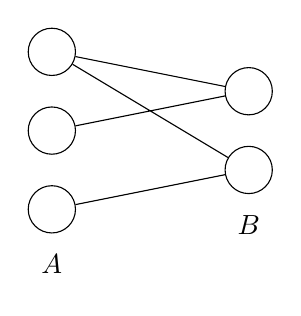
\begin{tikzpicture}[every node/.style={circle,draw,fill=white,inner sep=1.5pt,minimum size=6mm}]
\node (a1) at (0,1.5) {};
\node (a2) at (0,0.5) {};
\node (a3) at (0,-0.5) {};
\node (b1) at (2.5,1) {};
\node (b2) at (2.5,0) {};
\draw (a1)--(b1) (a1)--(b2) (a2)--(b1) (a3)--(b2);
\node[draw=none,fill=none] at (0,-1.2) {$A$};
\node[draw=none,fill=none] at (2.5,-0.7) {$B$};
\end{tikzpicture}
\end{center}
\begin{center}
\small A bipartite graph: every edge crosses between $A$ and $B$
\end{center}

\begin{definition}[$2$-colouring]
A \emph{$2$-colouring} of $G$ is a function $f:V\to\{\text{Black},\text{White}\}$ such that adjacent vertices get different colours.
\end{definition}

\begin{proposition}
$G$ is bipartite if and only if $G$ has a $2$-colouring.
\end{proposition}
\begin{proof}
($\Rightarrow$) Colour $A$ Black and $B$ White. Every edge goes between $A$ and $B$, so its endpoints get different colours.

($\Leftarrow$) Given a $2$-colouring $f$, let $A=f^{-1}(\text{Black})$ and $B=f^{-1}(\text{White})$. These split $V$ into two parts, and every edge joins differently coloured vertices, i.e.\ one in $A$ and one in $B$.
\end{proof}

\bigskip
\begin{theorem}
$G$ is bipartite if and only if $G$ has no closed walk of odd length.
\end{theorem}
\begin{proof}
($\Rightarrow$) A walk in a bipartite graph alternates sides $A,B,A,B,\dots$, so it can only return to its starting side after an even number of steps.

($\Leftarrow$) We build a $2$-colouring, one component at a time. In each component fix a vertex $g$, and colour $v$ Black if $d(g,v)$ is even and White if it is odd. Suppose, for contradiction, that some edge $\{v,w\}$ has both ends the same colour, so $d(g,v)$ and $d(g,w)$ have the same parity. Then a shortest path from $g$ to $v$, the edge $\{v,w\}$, and a shortest path from $w$ back to $g$ together form a closed walk of length $d(g,v)+d(g,w)+1$, which is odd. This contradicts the hypothesis, so the colouring is valid.
\end{proof}

\begin{corollary}
$G$ is bipartite if and only if $G$ has no cycle of odd length.
\end{corollary}
\begin{proof}
Combine the previous theorem with Theorem~\ref{thm:odd-closed-walk}.
\end{proof}

\begin{example}
$C_n$ is bipartite exactly when $n$ is even. $K_3$ (a triangle) is not bipartite, and neither is any graph containing a triangle.
\end{example}

\subsection{Euler tours and Hamiltonian cycles}
\label{sec:11-11}
% CN 11.11

\begin{definition}[Euler tour]
An \emph{Euler tour} of $G$ is a closed trail that uses every edge of $G$ exactly once. A graph with an Euler tour is \emph{Eulerian}.
\end{definition}

\begin{example}
A postal worker who wants to walk along every street exactly once and finish where they started is looking for an Euler tour of the street graph.
\end{example}

\begin{theorem}[Euler, 1736]
A connected graph $G$ has an Euler tour if and only if every vertex has even degree.
\end{theorem}
\begin{proof}
($\Rightarrow$) Follow the tour. Each time it passes through a vertex it uses two of that vertex's edges, one to arrive and one to leave; the first and last edges at the starting vertex also pair up in this way. Every edge is used exactly once, so each degree is a sum of $2$'s, hence even.

($\Leftarrow$) Start at any vertex and keep walking along unused edges. Whenever we arrive at a vertex other than the start, we have used an odd number of its edges, and its degree is even, so an unused edge remains to leave by. Hence we can only get stuck at the start, and we obtain a closed trail $T$.

If $T$ uses every edge, we are done. Otherwise, because $G$ is connected, some vertex $u$ on $T$ has an unused edge. (Take a path from a vertex of $T$ to an endpoint of any unused edge; the first edge on it that is not in $T$ starts at a vertex of $T$.) Since $T$ uses an even number of edges at each vertex, every vertex still has an even number of unused edges. So the same walking argument, starting at $u$ and using only unused edges, gives a closed trail $U$. Splicing $U$ into $T$ at $u$ gives a longer closed trail. Repeating this, the trail grows until it uses every edge.
\end{proof}

\begin{note}[Königsberg]
The four land masses of Königsberg are vertices and its seven bridges are edges. Every vertex has odd degree, so by the theorem there is no walk crossing every bridge exactly once and returning home, settling the old puzzle.
\end{note}

\begin{center}
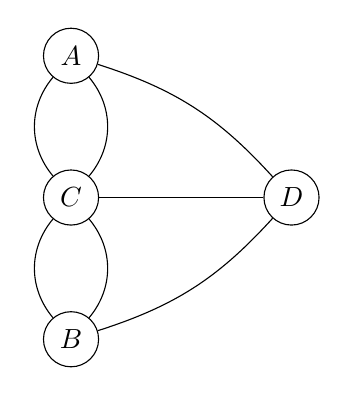
\begin{tikzpicture}[every node/.style={circle,draw,fill=white,inner sep=1.5pt,minimum size=7mm}]
\node (A) at (0,1.8) {$A$};
\node (B) at (0,-1.8) {$B$};
\node (C) at (0,0) {$C$};
\node (D) at (2.8,0) {$D$};
\draw (A) to[bend left=40] (C);
\draw (A) to[bend right=40] (C);
\draw (B) to[bend left=40] (C);
\draw (B) to[bend right=40] (C);
\draw (C)--(D);
\draw (A) to[bend left=15] (D);
\draw (B) to[bend right=15] (D);
\end{tikzpicture}
\end{center}
\begin{center}
\small Königsberg: the island $C$ has degree $5$, and $A$, $B$, $D$ have degree $3$, so no Euler tour exists
\end{center}

\begin{note}[Multigraphs]
The theorem also holds for multigraphs, and for graphs with loops if each loop counts $2$ towards the degree of its vertex.
\end{note}

\bigskip
\begin{theorem}[Route inspection / Chinese postman (extra)]
If $G$ is connected with $2k$ vertices of odd degree ($k\ge1$; this number is even by Corollary~\ref{cor:odd-degree}), then pairing them up and adding $k$ new edges, one per pair (parallel edges allowed), makes every degree even. The new graph therefore has an Euler tour.
\end{theorem}

\begin{note}[Re-using the fewest edges]
In practice the added edges stand for streets walked twice. Choosing the pairing so that the total re-walked length is as small as possible is the \emph{route inspection problem}. Unlike TSP (\S\ref{sec:11-8}), it can be solved efficiently.
\end{note}

\bigskip
\begin{definition}[Hamiltonian cycle]
\label{def:hamiltonian}
A cycle is \emph{Hamiltonian} if it contains every vertex of the graph.
\end{definition}

\begin{example}
$C_n$ and $K_n$ ($n\ge3$) have Hamiltonian cycles. A path graph has none, since it has no cycle at all. $K_{2,3}$ has none: a cycle alternates between the two sides, so it uses equally many vertices from each, but $2\ne3$.
\end{example}

\begin{theorem}[Dirac (extra)]
If $G$ is simple with $n\ge3$ vertices, and $\deg(v)\ge n/2$ for every $v$, then $G$ has a Hamiltonian cycle.
\end{theorem}

\begin{note}[Sufficient, not necessary]
Many Hamiltonian graphs fail Dirac's condition, e.g.\ $C_n$ for $n\ge5$, where every degree is $2$. The proof is beyond this unit.
\end{note}

\begin{definition}[Travelling Salesman Problem]
Given a weighted graph, find a Hamiltonian cycle of minimum total weight. (E.g.\ visit every city in a region exactly once and return home, as cheaply as possible.)
\end{definition}

\begin{proposition}
For $n\ge3$, $K_n$ has exactly $\dfrac{(n-1)!}{2}$ Hamiltonian cycles.
\end{proposition}
\begin{proof}
Fix a starting vertex. A Hamiltonian cycle is determined by the order in which the other $n-1$ vertices are visited, giving $(n-1)!$ orders. But each cycle is counted twice, once in each direction (and the two directions differ as $n\ge3$), so there are $(n-1)!/2$ cycles.
\end{proof}

\begin{note}[Why TSP is hard]
Checking every Hamiltonian cycle of $K_n$ means checking $(n-1)!/2$ cycles, which grows faster than any exponential. No efficient algorithm for TSP is known.
\end{note}

\subsection{Trees}
\label{sec:12-1}
% CN 12.1

\begin{definition}[Tree]
A \emph{tree} is a connected graph with no cycles.
\end{definition}

\begin{center}
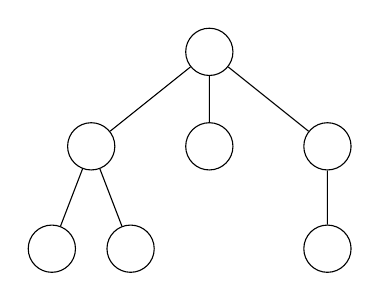
\begin{tikzpicture}[every node/.style={circle,draw,fill=white,inner sep=1.5pt,minimum size=6mm}]
\node (r) at (2,3) {};
\node (a) at (0.5,1.8) {};
\node (b) at (2,1.8) {};
\node (c) at (3.5,1.8) {};
\node (d) at (0,0.5) {};
\node (e) at (1,0.5) {};
\node (f) at (3.5,0.5) {};
\draw (r)--(a) (r)--(b) (r)--(c) (a)--(d) (a)--(e) (c)--(f);
\end{tikzpicture}
\end{center}
\begin{center}
\small A tree
\end{center}

\begin{note}[Where trees appear]
Trees model communication networks with the fewest possible links, hierarchies (directories, class inheritance, organisation charts), decision processes, and the structure of sentences in a grammar. Many of these have a special vertex called the \emph{root}, such as \texttt{/} in a Unix directory tree.
\end{note}

\subsection{Properties of trees}
\label{sec:12-2}
% CN 12.2

\begin{definition}[Minimal connected graph]
A connected graph $G$ is \emph{minimal connected} if deleting any one of its edges disconnects it.
\end{definition}

\begin{theorem}[CN Thm 66]
A graph $G$ is a tree if and only if it is a minimal connected graph.
\end{theorem}
\begin{proof}
($\Rightarrow$) Let $G$ be a tree, and suppose, for contradiction, that some edge $e=\{v,w\}$ can be deleted without disconnecting $G$. Then there is a path from $v$ to $w$ avoiding $e$, and adding $e$ to it gives a cycle, contradicting that $G$ has no cycles.

($\Leftarrow$) Let $G$ be minimal connected, and suppose, for contradiction, that $G$ has a cycle $C$; let $e$ be an edge of $C$. Any walk that uses $e$ can go the other way around $C$ instead, so deleting $e$ leaves the graph connected. This contradicts minimality.
\end{proof}

\begin{note}[Unique paths]
It follows that any two vertices of a tree are joined by exactly one path: two different paths would together contain a cycle.
\end{note}

\begin{note}[The two extreme trees]
Among trees on $n$ vertices, the path $P_{n-1}$ has the longest possible path (length $n-1$) and the smallest possible maximum degree ($2$). The star $K_{1,n-1}$ has the shortest paths (length at most $2$) and the largest possible maximum degree ($n-1$).
\end{note}

\begin{center}
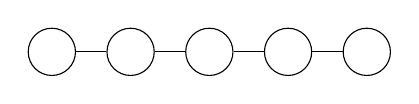
\begin{tikzpicture}[every node/.style={circle,draw,fill=white,inner sep=1.5pt,minimum size=6mm}]
\node (p1) at (0,0) {};
\node (p2) at (1,0) {};
\node (p3) at (2,0) {};
\node (p4) at (3,0) {};
\node (p5) at (4,0) {};
\draw (p1)--(p2)--(p3)--(p4)--(p5);
\end{tikzpicture}
\qquad
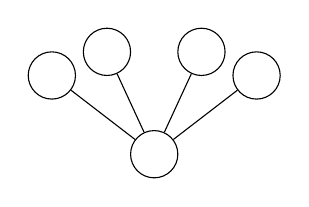
\begin{tikzpicture}[every node/.style={circle,draw,fill=white,inner sep=1.5pt,minimum size=6mm}]
\node (s0) at (0,0) {};
\node (s1) at (-1.3,1) {};
\node (s2) at (-0.6,1.3) {};
\node (s3) at (0.6,1.3) {};
\node (s4) at (1.3,1) {};
\draw (s0)--(s1) (s0)--(s2) (s0)--(s3) (s0)--(s4);
\end{tikzpicture}
\end{center}
\begin{center}
\small $P_4$ (left) and $K_{1,4}$ (right): the two extreme trees on $5$ vertices
\end{center}

\bigskip
\begin{theorem}[CN Thm 67]
Every tree with at least two vertices has a leaf.
\end{theorem}
\begin{proof}
Take a longest path $v_0,\dots,v_k$ in the tree; $k\ge1$ since there is at least one edge. Any neighbour of $v_k$ other than $v_{k-1}$ is either on the path, giving a cycle, or off it, giving a longer path. Neither is possible, so $\deg(v_k)=1$.
\end{proof}

\begin{theorem}[CN Thm 68]
For every $n\in\N$, every tree on $n$ vertices has $n-1$ edges.
\end{theorem}
\begin{proof}
We use induction on $n$.

\textbf{Base case} ($n=1$): The only tree on one vertex has $0=1-1$ edges.

\textbf{Inductive step}: Let $k\ge1$ and assume every tree on $k$ vertices has $k-1$ edges. Let $T$ be a tree on $k+1$ vertices. By CN Thm 67, $T$ has a leaf $\ell$. Deleting $\ell$ and its one edge gives a graph $S$ that is still connected (no path between other vertices passes through a leaf) and still has no cycles, so $S$ is a tree on $k$ vertices. By the inductive hypothesis $S$ has $k-1$ edges, so $T$ has $(k-1)+1=k$ edges.

By the Principle of Mathematical Induction, the claim holds for all $n$.
\end{proof}

\begin{note}[Using the edge count]
So a connected graph on $n$ vertices has at least $n-1$ edges, and has exactly $n-1$ if and only if it is a tree.
\end{note}

\subsection{Forests}
\label{sec:12-3}
% CN 12.3

\begin{definition}[Forest]
A \emph{forest} is a graph with no cycles (not necessarily connected).
\end{definition}

\begin{note}[A forest is a union of trees]
Each component of a forest is connected and has no cycles, so it is a tree.
\end{note}

\begin{theorem}[CN Thm 69]
For every $n\in\N$, every forest with $n$ vertices and $k$ components has $n-k$ edges.
\end{theorem}
\begin{proof}
Let the components be $F_1,\dots,F_k$, with $n_i$ vertices and $m_i$ edges. Each $F_i$ is a tree, so $m_i=n_i-1$ by CN Thm 68. Hence the number of edges is $\sum_i m_i = \sum_i (n_i-1) = n-k$.
\end{proof}

\begin{center}
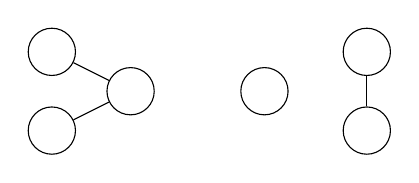
\begin{tikzpicture}[every node/.style={circle,draw,fill=white,inner sep=1.5pt,minimum size=6mm}]
\node (a) at (0,1) {}; \node (b) at (0,0) {}; \node (c) at (1,0.5) {};
\draw (a)--(c) (b)--(c);
\node (e) at (2.7,0.5) {};
\node (f) at (4,1) {}; \node (g) at (4,0) {};
\draw (f)--(g);
\end{tikzpicture}
\end{center}
\begin{center}
\small A forest with $k=3$ components: $n=6$ vertices and $3=n-k$ edges
\end{center}

\subsection{Spanning trees}
\label{sec:12-4}
% CN 12.4

\begin{definition}[Spanning tree]
A \emph{spanning tree} of a connected graph $G$ is a subgraph of $G$ that is a tree and contains every vertex of $G$.
\end{definition}

\begin{proposition}[Existence]
Every connected graph has a spanning tree.
\end{proposition}
\begin{proof}
Delete edges one at a time, each time choosing an edge whose deletion leaves the graph connected, until no such edge remains. The result is connected, contains every vertex, and is minimal connected, so it is a tree by CN Thm 66.
\end{proof}

\begin{example}
The graph below (the graph of \S\ref{sec:11-8}) has $6$ vertices and $8$ edges, so a spanning tree is obtained by deleting $3$ edges. Deleting $\{a,b\}$, $\{b,c\}$, $\{b,e\}$, each time keeping the graph connected, leaves the spanning tree drawn thick. Deleting $\{a,b\}$, $\{c,d\}$, $\{b,e\}$ instead gives a different spanning tree. Every spanning tree has $6-1=5$ edges.
\end{example}

\begin{center}
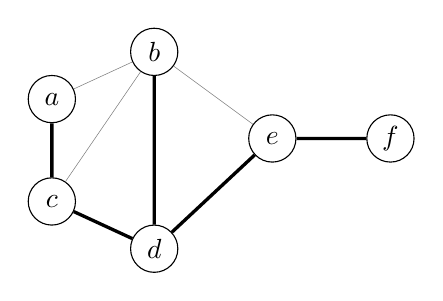
\begin{tikzpicture}[every node/.style={circle,draw,fill=white,inner sep=1.5pt,minimum size=6mm}]
\node (a) at (0,1) {$a$};
\node (b) at (1.3,1.6) {$b$};
\node (c) at (0,-0.3) {$c$};
\node (d) at (1.3,-0.9) {$d$};
\node (e) at (2.8,0.5) {$e$};
\node (f) at (4.3,0.5) {$f$};
\draw[very thin, gray] (a)--(b) (b)--(c) (b)--(e);
\draw[very thick] (a)--(c) (c)--(d) (b)--(d) (d)--(e) (e)--(f);
\end{tikzpicture}
\end{center}
\begin{center}
\small A spanning tree (thick edges)
\end{center}

\begin{note}[Building up instead]
Equivalently, start with no edges and repeatedly add any edge that does not create a cycle, until no more can be added:
\end{note}

\begin{algorithm}[H]
\SetAlgoLined
\KwIn{Connected graph $G=(V,E)$}
\KwOut{Spanning tree $F=(V,X)$}
$X\gets\emptyset$\;
\While{$\exists e\in E\setminus X$ such that $X\cup\{e\}$ has no cycle}{
    pick such an $e$\;
    $X\gets X\cup\{e\}$\;
}
\caption{Spanning tree by adding edges}
\end{algorithm}

\begin{proof}[Correctness]
$F$ has no cycle by construction. If $F$ were not connected, then since $G$ is connected some edge of $G$ would join two different components of $F$; adding it creates no cycle, so the algorithm would not have stopped. Hence $F$ is a connected graph with no cycles containing every vertex, i.e.\ a spanning tree.
\end{proof}

\bigskip
\begin{definition}[Minimum spanning tree]
In a connected graph with a weight (cost) $w(e)$ on each edge, a \emph{minimum spanning tree} is a spanning tree whose total weight $\sum_{e\in X}w(e)$ is as small as possible.
\end{definition}

\begin{algorithm}[H]
\SetAlgoLined
\KwIn{Connected weighted graph $G=(V,E,w)$}
\KwOut{Minimum spanning tree $F=(V,X)$}
$X\gets\emptyset$\;
\While{$\exists e\in E\setminus X$ such that $X\cup\{e\}$ has no cycle}{
    $e\gets$ such an edge of minimum weight\;
    $X\gets X\cup\{e\}$\;
}
\caption{Kruskal's Greedy Algorithm}
\end{algorithm}

\begin{theorem}[CN Thm 70]
For every weighted graph $G$, Kruskal's Greedy Algorithm finds a minimum weight spanning tree of $G$.
\end{theorem}

\begin{note}[Proof idea: the exchange argument]
CN does not prove this. The idea: suppose Kruskal's tree $T$ is not minimum, and let $T^*$ be a minimum spanning tree sharing as many edges with $T$ as possible. Let $e$ be the first edge chosen by Kruskal that is not in $T^*$. Adding $e$ to $T^*$ creates a cycle, which contains an edge $f\notin T$. When Kruskal chose $e$, the edge $f$ was also available (adding it would not have created a cycle), so $w(e)\le w(f)$. Then $T^*-f+e$ is a spanning tree of weight at most $w(T^*)$, so it is also minimum, and it shares more edges with $T$, a contradiction.
\end{note}

\begin{note}[Greedy is usually not optimal]
Repeatedly taking the biggest immediate benefit seldom gives the best overall result. For example, greedily following the shortest available edge does not, in general, find a shortest path between two vertices, and may not find a path at all. Minimum spanning trees are a striking exception.
\end{note}

\subsection{Planarity}
\label{sec:12-5}
% CN 12.5

\begin{definition}[Planar graph]
A graph is \emph{planar} if it can be drawn in the plane with no crossings: vertices are distinct points, and edges are curves that meet only at shared endpoints. Such a drawing is a \emph{plane graph}.
\end{definition}

\begin{note}[Why planarity matters]
Electrical circuits are laid out on flat circuit boards, and wires that cross can cause short circuits; maps and diagrams are easier to read without crossings.
\end{note}

\begin{definition}[Face]
A plane graph divides the plane into regions called \emph{faces}: each face is a maximal set of points any two of which can be joined by a curve avoiding all vertices and edges. The unbounded region is the \emph{outer face}, and it must be counted too.
\end{definition}

\begin{note}[Sides of an edge]
Walking around the boundary of every face, each edge is met exactly twice: once from each side. The two sides usually belong to different faces, but may belong to the same face (e.g.\ for an edge to a leaf).
\end{note}

\begin{center}
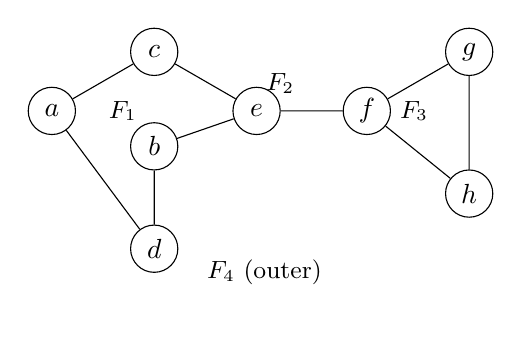
\begin{tikzpicture}[every node/.style={circle,draw,fill=white,inner sep=1.5pt,minimum size=6mm}]
\node (a) at (0,0.75) {$a$};
\node (b) at (1.3,0.3) {$b$};
\node (c) at (1.3,1.5) {$c$};
\node (d) at (1.3,-1) {$d$};
\node (e) at (2.6,0.75) {$e$};
\node (f) at (4,0.75) {$f$};
\node (g) at (5.3,1.5) {$g$};
\node (h) at (5.3,-0.3) {$h$};
\draw (a)--(c) (a)--(d) (c)--(e) (b)--(d) (b)--(e) (e)--(c) (e)--(f) (f)--(g) (f)--(h) (g)--(h);
\node[draw=none,fill=none] at (0.9,0.75) {\small $F_1$};
\node[draw=none,fill=none] at (2.9,1.1) {\small $F_2$};
\node[draw=none,fill=none] at (4.6,0.75) {\small $F_3$};
\node[draw=none,fill=none] at (2.7,-1.3) {\small $F_4$ (outer)};
\end{tikzpicture}
\end{center}
\begin{center}
\small A plane graph with $n=8$, $m=10$, $f=4$; indeed $n-m+f=8-10+4=2$
\end{center}

\bigskip
\begin{theorem}[Euler's Theorem, CN Thm 71]
Let $G$ be a connected plane graph with $n$ vertices, $m$ edges and $f$ faces. Then $n-m+f = 2$.
\end{theorem}
\begin{proof}
Fix $n$; we use induction on $m$. Since $G$ is connected, $m\ge n-1$.

\textbf{Base case} ($m=n-1$): $G$ is a connected graph with $n-1$ edges, so it is a tree. A tree has no cycle to enclose a region, so $f=1$, and $n-(n-1)+1=2$.

\textbf{Inductive step}: Let $m\ge n-1$ and assume the formula for connected plane graphs with $n$ vertices and $m$ edges. Let $G$ have $n$ vertices, $m+1$ edges and $f$ faces. Since $m+1>n-1$, $G$ is not a tree, so it has a cycle; let $e$ be an edge on it. The cycle separates the plane, so the two sides of $e$ lie in different faces. Deleting $e$ keeps the graph connected and merges those two faces into one, giving $H$ with $n$ vertices, $m$ edges and $f-1$ faces. By the inductive hypothesis $n-m+(f-1)=2$, that is, $n-(m+1)+f=2$.

By the Principle of Mathematical Induction, the formula holds for all $m\ge n-1$.
\end{proof}

\begin{corollary}[CN Cor 72]
For any simple planar graph with $n\ge3$ vertices and $m$ edges, \ $m \le 3n-6$.
\end{corollary}
\begin{proof}
We may assume $G$ is connected, since adding edges between components keeps it planar and only increases $m$. Take a plane drawing with $f$ faces. Since $G$ is simple with $n\ge3$, every face has at least $3$ sides, and every edge has exactly $2$ sides, so $3f\le2m$. By Euler's Theorem, $2=n-m+f\le n-m+\frac23m=n-\frac13m$, which rearranges to $m\le3n-6$.
\end{proof}

\begin{corollary}[CN Cor 73]
$K_5$ is nonplanar.
\end{corollary}
\begin{proof}
$K_5$ has $n=5$ and $m=10$, but $3n-6=9<10$, contradicting CN Cor 72.
\end{proof}

\begin{corollary}[CN Cor 74]
For any triangle-free simple planar graph with $n\ge3$ vertices and $m$ edges, \ $m\le2n-4$.
\end{corollary}
\begin{proof}
As for CN Cor 72, but now every face has at least $4$ sides, so $4f\le2m$. Then $2=n-m+f\le n-m+\frac12m$, giving $m\le2n-4$.
\end{proof}

\begin{corollary}[CN Cor 75]
$K_{3,3}$ is nonplanar.
\end{corollary}
\begin{proof}
$K_{3,3}$ is bipartite, so it has no odd cycles and in particular no triangles. It has $n=6$ and $m=9$, but $2n-4=8<9$, contradicting CN Cor 74.
\end{proof}

\begin{note}[A crossing drawing does not prove nonplanarity]
A graph may have drawings with crossings and still be planar. $K_4$ is planar, as the second drawing below shows; to prove a graph \emph{non}planar, use a counting argument like the ones above.
\end{note}

\begin{center}
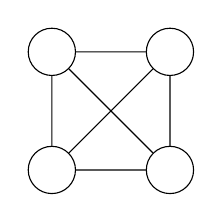
\begin{tikzpicture}[every node/.style={circle,draw,fill=white,inner sep=1.5pt,minimum size=6mm}]
\node (a) at (0,1.5) {};
\node (b) at (1.5,1.5) {};
\node (c) at (0,0) {};
\node (d) at (1.5,0) {};
\draw (a)--(b) (a)--(c) (a)--(d) (b)--(c) (b)--(d) (c)--(d);
\end{tikzpicture}
\qquad
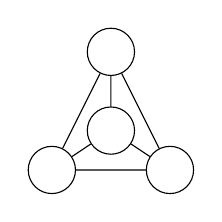
\begin{tikzpicture}[every node/.style={circle,draw,fill=white,inner sep=1.5pt,minimum size=6mm}]
\node (a) at (0.75,2) {};
\node (b) at (0,0.5) {};
\node (c) at (1.5,0.5) {};
\node (d) at (0.75,1) {};
\draw (a)--(b) (a)--(c) (a)--(d) (b)--(c) (b)--(d) (c)--(d);
\end{tikzpicture}
\end{center}
\begin{center}
\small $K_4$: a drawing with a crossing (left) and a plane drawing (right) of the same graph
\end{center}

\begin{theorem}[Four colour theorem (extra)]
The vertices of every planar graph can be coloured with $4$ colours so that adjacent vertices get different colours.
\end{theorem}

\begin{note}[History]
Conjectured in 1852 and proved in 1976 by Appel and Haken. It was the first major theorem whose proof essentially needed a computer (to check about $1900$ configurations), which was controversial because no person could check it by hand.
\end{note}

\subsection{Games on graphs}
\label{sec:12-6}
% CN 12.6

\subsubsection{Shannon's Switching Game}
\label{sec:12-6-1}
% CN 12.6.1

\begin{definition}[Shannon's Switching Game]
The game is played on a connected graph $G$ with two \emph{terminals} $s,t$. Two players, \emph{Join} and \emph{Cut}, take turns. Join thickens an edge that is not yet crossed out; Cut crosses out an edge that is not yet thickened. Join wins as soon as the thickened edges contain a path from $s$ to $t$. Cut wins as soon as $s$ and $t$ are in different components of the graph of edges not crossed out.
\end{definition}

\begin{center}
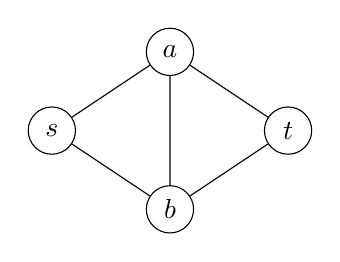
\begin{tikzpicture}[every node/.style={circle,draw,fill=white,inner sep=1.5pt,minimum size=6mm}]
\node (s) at (0,0) {$s$};
\node (a) at (1.5,1) {$a$};
\node (b) at (1.5,-1) {$b$};
\node (t) at (3,0) {$t$};
\draw (s)--(a) (s)--(b) (a)--(t) (b)--(t) (a)--(b);
\end{tikzpicture}
\end{center}

\begin{example}
On the graph above, with Join first: Join thickens $\{s,a\}$; Cut crosses out $\{a,t\}$; Join thickens $\{a,b\}$; Cut crosses out $\{b,t\}$. Now $s$ and $t$ are separated, so Cut wins. Join's second move was a blunder: thickening $\{b,t\}$ instead would have threatened both $s,b,t$ and $s,a,b,t$, and Cut cannot block both.
\end{example}

\begin{proposition}[No draws]
Every play of Shannon's Switching Game ends with a winner.
\end{proposition}
\begin{proof}
If play continued until every edge were thickened or crossed out, then the thickened edges would either contain a path from $s$ to $t$, so Join wins, or not, in which case $s$ and $t$ are separated in the graph of remaining edges, so Cut wins. So the game always ends with a winner, possibly earlier.
\end{proof}

\begin{note}[Four possible cases]
Since there are no draws, on each graph exactly one of these holds: Join has a winning strategy whoever starts; Cut has a winning strategy whoever starts; the first player has a winning strategy; or the second player has a winning strategy. In fact the last case never happens.
\end{note}

\bigskip
\begin{theorem}[The second player never has the advantage]
There is no graph on which the second player has a winning strategy whichever role they play.
\end{theorem}
\begin{proof}
We use strategy stealing. Suppose, for contradiction, that on some graph the second player has a winning strategy $\sigma$, whichever role they play. The first player makes an arbitrary first move, and then plays as if they were the second player following $\sigma$, ignoring their extra move. In this game an extra thickened (or crossed-out) edge never hurts its owner, so the first player still wins, as $\sigma$ guarantees. But then the second player's $\sigma$ is not a winning strategy, a contradiction.
\end{proof}

\begin{note}[Bridg-It]
A commercial version of this game, Bridg-It, was invented by David Gale and sold from 1960.
\end{note}

\subsubsection{Slither}
\label{sec:12-6-2}
% CN 12.6.2

\begin{definition}[Slither]
Two players take turns choosing edges so that the chosen edges always form a path. The first move is any edge. Each later edge must have one endpoint at either end of the current path and its other endpoint not yet on the path. The first player who cannot move loses.
\end{definition}

\begin{note}[Impartial vs.\ partisan]
In Slither both players make the same kind of move, so the game is \emph{impartial}; Shannon's Switching Game, where one player thickens and the other crosses out, is \emph{partisan}. Unlike Shannon's game, Slither has graphs where the first player has a winning strategy and also graphs where the second player does.
\end{note}

